\documentclass[10pt,landscape,a4paper]{article}
\usepackage[utf8]{inputenc}
\usepackage[ngerman]{babel}
\usepackage{tikz}
\usetikzlibrary{shapes,positioning,arrows,fit,calc,graphs,graphs.standard}
\usepackage[nosf]{kpfonts}
\usepackage[t1]{sourcesanspro}
%\usepackage[lf]{MyriadPro}
%\usepackage[lf,minionint]{MinionPro}
\usepackage{multicol}
\usepackage{wrapfig}
\usepackage[top=0mm,bottom=1mm,left=0mm,right=1mm]{geometry}
\usepackage[framemethod=tikz]{mdframed}
\usepackage{microtype}

\graphicspath{{Images/}}

\DeclareMathOperator*{\argmin}{arg\,min}
\DeclareMathOperator*{\argmax}{arg\,max}
\newcommand{\vek}[1]{\mathbf{#1}}
\newcommand*{\vertbar}{\rule[-1ex]{0.5pt}{2.5ex}}
\newcommand*{\horzbar}{\rule[.5ex]{2.5ex}{0.5pt}}
\newcommand\independent{\protect\mathpalette{\protect\independenT}{\perp}}
\def\independenT#1#2{\mathrel{\rlap{$#1#2$}\mkern2mu{#1#2}}}


\let\bar\overline

\definecolor{myblue}{cmyk}{1,.72,0,.38}

\def\firstcircle{(0,0) circle (1.5cm)}
\def\secondcircle{(0:2cm) circle (1.5cm)}

\colorlet{circle edge}{myblue}
\colorlet{circle area}{myblue!5}

\tikzset{filled/.style={fill=circle area, draw=circle edge, thick},
    outline/.style={draw=circle edge, thick}}

\pgfdeclarelayer{background}
\pgfsetlayers{background,main}

\everymath\expandafter{\the\everymath \color{myblue}}
\everydisplay\expandafter{\the\everydisplay \color{myblue}}

\renewcommand{\baselinestretch}{.8}
\pagestyle{empty}

\global\mdfdefinestyle{header}{%
linecolor=gray,linewidth=1pt,%
leftmargin=0mm,rightmargin=0mm,skipbelow=0mm,skipabove=0mm,
}

\newcommand{\header}{
\begin{mdframed}[style=header]
\footnotesize
\sffamily
COMP 652 - Machine Learning\\
by~Carlos G. Oliver,~page~\thepage~of~2
\end{mdframed}
}

\makeatletter
\renewcommand{\section}{\@startsection{section}{1}{0mm}%
                                {.2ex}%
                                {.2ex}%x
                                {\color{myblue}\sffamily\small\bfseries}}
\renewcommand{\subsection}{\@startsection{subsection}{1}{0mm}%
                                {.2ex}%
                                {.2ex}%x
                                {\sffamily\bfseries}}



\def\multi@column@out{%
   \ifnum\outputpenalty <-\@M
   \speci@ls \else
   \ifvoid\colbreak@box\else
     \mult@info\@ne{Re-adding forced
               break(s) for splitting}%
     \setbox\@cclv\vbox{%
        \unvbox\colbreak@box
        \penalty-\@Mv\unvbox\@cclv}%
   \fi
   \splittopskip\topskip
   \splitmaxdepth\maxdepth
   \dimen@\@colroom
   \divide\skip\footins\col@number
   \ifvoid\footins \else
      \leave@mult@footins
   \fi
   \let\ifshr@kingsaved\ifshr@king
   \ifvbox \@kludgeins
     \advance \dimen@ -\ht\@kludgeins
     \ifdim \wd\@kludgeins>\z@
        \shr@nkingtrue
     \fi
   \fi
   \process@cols\mult@gfirstbox{%
%%%%% START CHANGE
\ifnum\count@=\numexpr\mult@rightbox+2\relax
          \setbox\count@\vsplit\@cclv to \dimexpr \dimen@-1cm\relax
\setbox\count@\vbox to \dimen@{\vbox to 1cm{\header}\unvbox\count@\vss}%
\else
      \setbox\count@\vsplit\@cclv to \dimen@
\fi
%%%%% END CHANGE
            \set@keptmarks
            \setbox\count@
                 \vbox to\dimen@
                  {\unvbox\count@
                   \remove@discardable@items
                   \ifshr@nking\vfill\fi}%
           }%
   \setbox\mult@rightbox
       \vsplit\@cclv to\dimen@
   \set@keptmarks
   \setbox\mult@rightbox\vbox to\dimen@
          {\unvbox\mult@rightbox
           \remove@discardable@items
           \ifshr@nking\vfill\fi}%
   \let\ifshr@king\ifshr@kingsaved
   \ifvoid\@cclv \else
       \unvbox\@cclv
       \ifnum\outputpenalty=\@M
       \else
          \penalty\outputpenalty
       \fi
       \ifvoid\footins\else
         \PackageWarning{multicol}%
          {I moved some lines to
           the next page.\MessageBreak
           Footnotes on page
           \thepage\space might be wrong}%
       \fi
       \ifnum \c@tracingmulticols>\thr@@
                    \hrule\allowbreak \fi
   \fi
   \ifx\@empty\kept@firstmark
      \let\firstmark\kept@topmark
      \let\botmark\kept@topmark
   \else
      \let\firstmark\kept@firstmark
      \let\botmark\kept@botmark
   \fi
   \let\topmark\kept@topmark
   \mult@info\tw@
        {Use kept top mark:\MessageBreak
          \meaning\kept@topmark
         \MessageBreak
         Use kept first mark:\MessageBreak
          \meaning\kept@firstmark
        \MessageBreak
         Use kept bot mark:\MessageBreak
          \meaning\kept@botmark
        \MessageBreak
         Produce first mark:\MessageBreak
          \meaning\firstmark
        \MessageBreak
        Produce bot mark:\MessageBreak
          \meaning\botmark
         \@gobbletwo}%
   \setbox\@cclv\vbox{\unvbox\partial@page
                      \page@sofar}%
   \@makecol\@outputpage
     \global\let\kept@topmark\botmark
     \global\let\kept@firstmark\@empty
     \global\let\kept@botmark\@empty
     \mult@info\tw@
        {(Re)Init top mark:\MessageBreak
         \meaning\kept@topmark
         \@gobbletwo}%
   \global\@colroom\@colht
   \global \@mparbottom \z@
   \process@deferreds
   \@whilesw\if@fcolmade\fi{\@outputpage
      \global\@colroom\@colht
      \process@deferreds}%
   \mult@info\@ne
     {Colroom:\MessageBreak
      \the\@colht\space
              after float space removed
              = \the\@colroom \@gobble}%
    \set@mult@vsize \global
  \fi}

\makeatother
\setlength{\parindent}{0pt}

\begin{document}
\small
\begin{multicols*}{5}
%!TEX root = 652_cheatsheet.tex
\section{Math}
{\bf Bayes rule: } $P(A \vert B) = \frac{P(A, B)}{P(B)} = \frac{P(B \vert A) P(A)}{P(B)}$\\
$P(A,B \vert C) = \frac{P(A, B, C)}{P(C)}$ \\
{\bf Cond indep:} $P(A, B \vert C) = P(A \vert C)P(B \vert C)$\\
{\bf Chain rule: } $P(A_n, \ldots , A_1)  = \mathrm P(A_n | A_{n-1}, \ldots , A_1) \cdot\mathrm P( A_{n-1}, \ldots , A_1)$\\
{\bf Joint: } $\mathrm  P\left(\bigcap_{k=1}^n A_k\right)  = \prod_{k=1}^n  \mathrm P\left(A_k \,\Bigg|\, \bigcap_{j=1}^{k-1} A_j\right)$\\
{\bf Posterior:} unobserved $\theta$, observed $x$: $p(\theta \vert x) = \frac{p(x \vert \theta)p(\theta)}{p(x)}$\\
{\bf Prior:} prior belief in dist. of $\theta$: $p(\theta)$\\
{\bf Marginal: } $\Pr(X=x) = \sum_y \Pr(X=x,Y=y) = \sum_y \Pr(X=x\mid Y=y) \Pr(Y=y)$\\
{\bf Likelihood:} prob of observed given parameters: $p(x \vert \theta)$\\
{\bf Covariance:} $Cov(X,Y) = E\{(X - E(X))(Y- E(Y))\}$ \\
{\bf MAP:} $h_{MAP} = \argmax_{h\in H} P(h \vert D) = \argmax_{h\in H} P(D \vert h) P(h)$\\ 
{\bf Lagrange: } $L(\vek{x}, \lambda) = f(\vek{x}) + \lambda g(\vek{x})$
Set constraint $g(\vek{x})$ to zero and add multiplier. \\
{\bf Multinomial: } $(x_1 + x_2  + \cdots + x_m)^n 
 = \sum_{k_1+k_2+\cdots+k_m=n} {n \choose k_1, k_2, \ldots, k_m}
  \prod_{t=1}^m x_t^{k_t}\,$ \\
  $(a+b+c)^3 = a^3 + b^3 + c^3 + 3 a^2 b + 3 a^2 c + 3 b^2 a + 3 b^2 c + 3 c^2 a + 3 c^2 b + 6 a b c.$\\
{\bf Entropy: } $H(X)  = - \sum_{i=1}^n p(x_i)\log p(x_i)$\\
{\bf Cond. entropy:} $H(Y \vert X) = \sum_{x \in X} p(x) H(Y \vert X = x) = - \sum_{x \in X} p(x) \sum_{y \in Y}p(y \vert x) \log p(y \vert x) = \sum_{x \in X, y \in Y} p(x,y) \log \frac{p(x)}{p(x, y)}$\\
$H(Y \vert X) = H(X \vert Y) - H(X) + H(Y)$ 
$H(X_1, ... X_n) = \sum_{i}^{n} H(X_i \vert X_1, ... X_{n-1})$
{\bf KL Divergence: } $D_{KL} = \sum_{x} P(x) \log \frac{P(x)}{Q(x)}$ \\
{\bf Mutual info: } $I(X;Y) = \sum_{y \in Y}\sum_{x \in X} p(x,y) \log \frac{p(x, y)}{p(x)p(y)}$\\
$I(X;Y) = H(X) - H(X \vert Y) = H(X, Y) - H(X \vert Y) - H(Y \vert X)$
$$\vek{xy^T} = \begin{bmatrix}
           x_{1} \\
           \vdots \\
           x_{m}
         \end{bmatrix}      
         \begin{bmatrix}
           x_{1}\hdots x_{n}
         \end{bmatrix} = \begin{bmatrix}
         x_1 y_1 & \hdots & x_1 y_n \\
         \vdots & \ddots  & \vdots \\
          x_m y_1 & \hdots & x_m y_n \\
         \end{bmatrix}
         $$
{\bf Matrix-vector product: } $ \vek{Ax} = \begin{bmatrix}
 	a_1^T\vek{x}\\
	\vdots \\
	a_m^T\vek{x}
	\end{bmatrix}
$

{\bf Matrix mult': } $ (\mathbf{A}\mathbf{B})_{ij} = \sum_{k=1}^m A_{ik}B_{kj}\,$

$$ \vek{AB} =  \begin{bmatrix}
         a_1^Tb_1&  a_1^T b_2 & \hdots & a_1^T b_p \\
         \vdots & \vdots  & \ddots  & \vdots \\
          a_m^T b_1 & a_m^T b_2 & \hdots & a_m^T b_n \\
         \end{bmatrix}
$$

{\bf Multip'n dimensions: } $(n \times p)(p \times m) = n \times p$

$\sin(x)^{'} = \cos{x}$ \\
$\cos(x)^{'} = -\sin{x}$\\
$\sigma(x)^{'} = \sigma(x)(1-\sigma(x))$
$(AB)^{T} = B^{T}A$\\
$\log_{b}(x^{y}) = y \log_{b}(x)$\\
{\bf Unif: } $P_{\theta_1, \theta_2}(x) = \frac{1}{\theta_2 - \theta_1}$ \\
$AA^{-1} = A^{-1}A = I$ for square matrices. \\
{\bf Chain rule: } $F'(x) = f'(g(x)) g'(x)$ \\
{\bf Product rule: } $(f\cdot g)'=f'\cdot g+f\cdot g' \,\!$ \\
{\bf Norm: } $\vert \vert \vek{x} \vert \vert_{d} = \sum_{i} x_{i}^{d}$ \\
{\bf Bias vs Variance: } $\mathrm{E}\Big[\big(y - \hat{f}(x)\big)^2\Big] = \mathrm{E}\big[\hat{f}(x) - f(x)\big]^2 + \mathrm{E}[\hat{f}(x)^2] - \mathrm{E}[\hat{f}(x)]^2 + \epsilon^2$

%%%% EARLY STUFF %%%

\section{Regression}
\subsection{Regularization}
Higher $\lambda$ more bias. With more data, variance decreases can afford weaker regularization (less bias).
\subsection{L2 regularization}
Weights do not reach zero. Faster.
$$J_w = \frac{1}{2}(\Phi\vek{w} - \vek{y})^T(\Phi \vek{w} - \vek{y}) + \frac{\lambda}{2}\vek{w}^T\vek{w}$$
$$\vek{w} = (\Phi^T\Phi + \lambda \vek{I})^{-1}\Phi^Ty$$
\subsection{L1 regularization}
Some weights set to zero. More expensive. 
\subsection{Gradient Descent}
$\vek{w} \leftarrow \vek{w} - \alpha \nabla \log L(\vek{w})$
$\vek{w} \leftarrow \vek{w} - \alpha \nabla \log J(\vek{w})$
\subsection{Logistic Regression}
$\sigma (t) = \frac{e^t}{e^t+1} = \frac{1}{1+e^{-t}}$
$L(\mathbf{w}) =\ -\frac1N\sum_{n=1}^N\ \bigg[y_n  \log \hat y_n + (1 - y_n)  \log (1 - \hat y_n)\bigg]$

\subsection{Bayesian regularization}
Can sample hypotheses from prior distribution on parameters. When get data, posterior changes where we draw hypotheses from. No need for regularization. Use sequential bayesian updating to get new prior on parameters given data. $\text{new prior} \propto {current prior} \times {new likelihood}$ \\
i.e. $\pi_{n+1} \propto \pi_{n} \times p(x_{n+1} \vert \theta_n, x_n)$


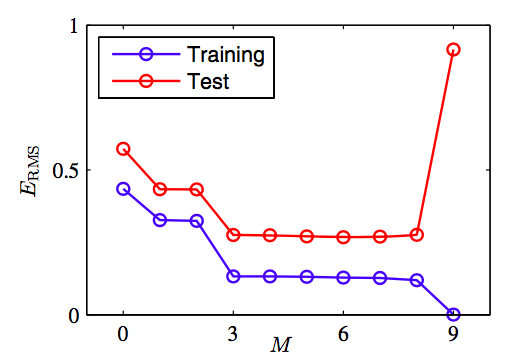
\includegraphics[width=0.5\linewidth]{error.png}

\section{Kernels}
$k(\vek{x}, \vek{z}) = \phi(\vek{x}) \cdot \phi(\vek{z})$
{\bf Mercer theorem:} $K(\vek{x}, \vek{z})$ is kernel iff Gram matrix $\vek{K}$ symmetric and positive semidefinite: $\vek{K_{ij}} = \vek{K_{ji}}$ and $\vek{z}^{T}\vek{K}\vek{z} \geq 0$
$\vek{K} = \Phi\Phi^T$ where $\vek{K_{nm}} = \phi(\vek{x_n})^T\phi(\vek{x_m}) = k(\vek{x_n}, \vek{x_m})$ Gram matrix size of input. Try to find a feature map whose dot product yields the kernel.


\section{SVM}
Minimize absolute error. More robust to outliers. Max margin is convex optimization.
$h_{\vek{w}}(\vek{x}) = \text{sign}(\sum_{i=1}^m \alpha_{i}y_{i}(\vek{x_{i}}\vek{x}) + \vek{w_0})$

$\alpha_{i} > 0$ only for support vectors. Soft error SVM: $0 < \zeta \leq 1$ if inside margin. $\zeta > 1$ if misclassified. Total errors: $C \sum_{i} \zeta$. Large $C$ higher variance.

\section{EM/Active Learning/Missing Data}
When missing data: many local maxima (normally likelihood has unique max), no closed form solutions. So we do gradient ascent or EM. $\log L(\theta) = \sum_{\text{complete data}} \log P(\vek{x_i}, y_i \vert \theta) + \sum_{\text{incomplete data}} \log \sum_{y} (\vek{x_i} \vert \theta)$. {\bf E step}: compute expected assignment (hard or soft, in soft we compute the weight for each distribution accounting for each point.) of points to distributions (estimate $p(y_i = k \vert \theta)$). {\bf M step: } recompute parameters to maximize likelihood of current assignments $p(\theta \vert y_i)$. Good for low dimensionality data. 
{\bf Active learning sampling strategies: } 1. generate examples for oracle. 2. query if instance in region of uncertainty (costly to maintain region) 3. uncertainty sampling. 4. query by committee (set of hypotheses vote. take examples for which KL divergence between distributions predicted by each hypothesis is high). 5. Expected error reduction/ max info gain (consider impact of labelling $\vek{x}$ with all labels, measure impact on other examples. 6. Density based (queries far from major concentration of data less useful)
\section{Bayes Nets}
$p(x_1, ..., x_{n}) = \prod_{i-1}^{n} p(x_i \vert x_{\pi_i})$

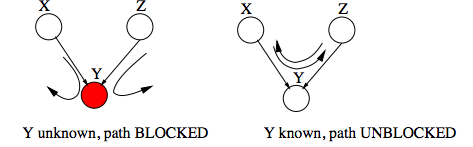
\includegraphics[width=0.5\linewidth]{path_1.png}
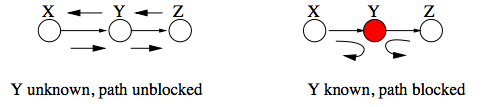
\includegraphics[width=0.5\linewidth]{path_2.png}
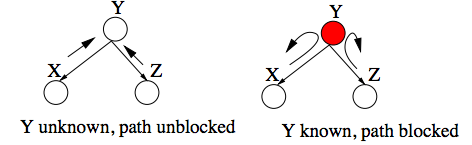
\includegraphics[width=0.5\linewidth]{path_3.png}
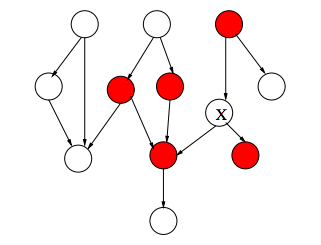
\includegraphics[width=0.3\linewidth]{markov_blanket.png}

{\bf Markov blanket: } parents, children, spouses. \\
{\bf Moral graph: } graph $U$: edge $(X, Y) \in U$ if $X$ in $Y$'s markov blanket. \\
{\bf Belief propagation: } This is exact inference $m_{ji} = \sum_{x_j} \bigg( \psi^E(x_j)\psi(x_i, x_j) \prod_{k \in \text{nghbr}(x_j)} m_{kj}(x_j)\bigg)$\\
$p(y \vert \hat{x}_{E}) \propto \psi^{E}(y) \prod_{k \in \text{nghbr}(Y)} m_{ky}(y)$

{\bf Gibbs Sampling (approximate inference):} 1. set evidence nodes $E = e$, all others random. 2. Sample $x_{i}'$ from $P(X_{i} \vert x_1, .., x_n)$ i.e. markov blanket. 3. Obtain new $x_{1}'..x_{n}'$. Converges to true steady state distribution using makov chain properties.\\
{\bf Learning: } likelihood of whole graph decomposes to likelihood over each node's parameter $L(\theta \vert D) = \prod_{i \in \text{nodes}}^{n} L(\theta_i \vert D)$. Use EM.
\section{Markov Chains}
{\bf Markov property: } $P(s_{t+1} \vert s_t) = P(s_{t+1} \vert s_0, .. s_t)$ \\
 $P(s_{t+1 = s'}) = \sum_s P(s_0 = s) P(s_1 = s' \vert s_0 = s)$ in matrix form: $\vek{p_t} = vek{T}^T \vek{p_{t-1}} = (\vek{T}^T)^t\vek{p_0}$ 
 
 \section{Hidden Markov Models}
 
 {\bf Parameters: } states, observations: $\mathcal{S, O}$,  $\vek{b_0}  \in | \mathcal{S} |$, transition probs $\vek{T} \in | \mathcal{S} | \times | \mathcal{S} |$, emission probs $\vek{Q} \in |\mathcal{S}| \times |\mathcal{O}|$ \\
 $P(o_1, ..,o_T, s_1, .., s_T) = P(s_1)P(o_1 \vert s_1) \prod_{t=2}^T P(s_t \vert s_{t-1})P(o_t \vert s_t)$\\
 {\bf Forward alg:} Compute $P(o_{1:t}, S_t=s, )$ $\alpha_t(S_t) = P(o_1,..,o_t, S_t = s) = \sum_{s_{t-1}}P(o_{t} \vert s_{t}) P(s_{t} \vert s_{t-1}) \alpha_{t-1}(s_{t-1}), \alpha_{t}(s_1) = P(o_1, s_1) = P(s_1)p(o_1 \vert s_1)$\\
 {\bf Backward alg: } obtain $\beta_{t}(s_t) = p(o_{t+1:n} \vert s_t)$. $\beta_{t}(s_t) = \sum_{s_{t+1}} \beta_{t+1}(s_{t+1}) P(o_{t+1} \vert s_{t+1}) P(s_{t+1} \vert s_t)$\\
 {\bf F-B alg: } 1. compute $\alpha_{t}(s)$. 2. compute $\beta_{t}(s)$ 3. for an $s$ and $t$: $P(S_t \vert o_1, ..., o_T) = \frac{P(o_1, .. o_T, S_t = s) P(o_{t+1}, ..., o_T \vert S_t = s)}{P(o_1, ..., o_T} = \frac{\alpha_{t}(s) \beta_{t}(s)}{\sum_{s'}\alpha_{T}(s')}$ Complexity: $O(|S|T)$\\
 {\bf Baum-Welch:} EM for missing parameters. Given obs. and initial parameters $\lambda = (\beta_0(s), p_{ss'}, q_{so})$. 1. (E-step) Compute $P(S_t \vert o_1,...o_T) \forall s, t$, $P(S_t =s, S_{t+1} = s' \vert o_1, ..., o_T) \forall s, s', t$ (using F-B, $O(|S|T + |S|^2T)$). 2. (M-step) $b_0(s) = P(S_1 = s \vert o_1, .., o_T)$, $p_{ss'} = \frac{\text{expected \# of s to s'}}{\text{expected s occurences}} = \frac{\sum_{t<T} P(S_t = s, S_{t+1} = s' \vert o_1, ..., o_T)}{ \sum_{t<T} P(S_t =s \vert o_1, ..., o_T)}$, $q_{so} = \frac{\text{expected \# of o from s}}{\text{expected s occurences}} = \frac{\sum_{t:o_t=o} P(S_t = s \vert o_1, ..., o_T)}{ \sum_{t} P(S_t =s \vert o_1, ..., o_T)}$, $O(|S|^2T + |S||O||T|)$\\
 
\section{Undirected Graphical Models}
$X \independent Z \vert Y$ if every path from $X$ to $Z$ goes through $Y$. Capture correlations, not causality. Can't always go from bayes to undirected and back. If two nodes not connected by arc, they are conditionally independent given rest of graph. Express joint as product of maximal clique potentials: $p(X_1 = x_1, ..., X_n=x_n) = \frac{1}{Z} \prod_{\text{cliques} C} \psi_C(\vek{x_C})$ where $\vek{x_C}$ is the values if nodes in $C$, and $Z = \sum_x \prod_{C} \psi_C(\vek{x_C})$. $\psi_C(\vek{x_C}) = e^{-H_C(\vek{x_C})}$ We define H to be anything. $p(\vek{x}) = Z^{-1}\prod_C e^{-H_C(\vek{x_C})} = Z^{-1} e^{-\sum_C H_C(\vek{x_C})} = Z^{-1} e^{-H(\vek{x})}$ where $H_C$ is the energy of the clique. For a 2D spin glass: $H(\vek{x}) = \sum_{i,j} \beta_{ij}x_i x_j + \sum_i \alpha_i x_i$ can do belief propagation like in bayes net with the messages. Order of updates is important. Potentials energy of agreement or disagreement in clique. \\
{\bf Parameter Learning: }  Because of normalization learning can't be broken down, can use gradient based. Max likelihood: $\log L(\psi \vert D) = \sum_{i=1}^N \log p(x_1^i, ... , x_n^i) = Z^{-1} \psi_C(\vek{x_C}) = (\sum_C \sum_{x_C} N(x_C)\log \psi_C(x_C)) - N \log Z$ for each clique, $N(x_C)$ are sufficient statistics. Take derivative and get $P_{ML} = \frac{N(x_C)}{N}$. At max $\frac{\hat{p}}{\psi_C(x_C)} = \frac{p}{\psi_C(x_C)}$ so we compute marginal under current guess $p^0(x_C)$ and recompute to get closer to equality above. $\psi^{t+1}_C(x_C) = \psi^{t}_{C}(x_C) \frac{\hat{p}(x_C)}{p^t(x_C)}$ Will converge in the limit. Need initial guess $\psi^0$.

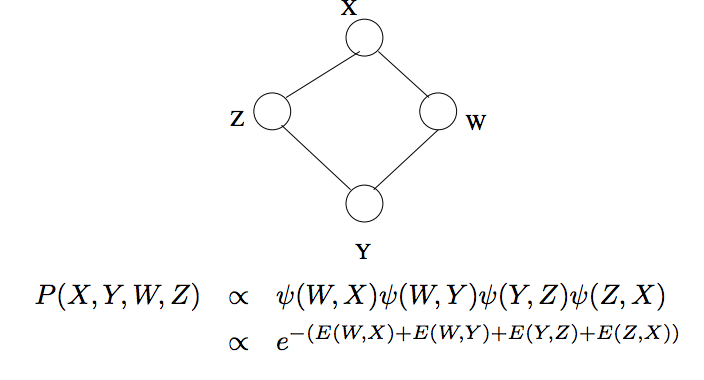
\includegraphics[width=0.5\linewidth]{mrf.png}

\section{PCA}
Try to minimize reconstruction error.
{\bf Kernel PCA:} 1. pick kernel 2. Construct normalized kernel matrix $\vek{\tilde{K}} \in m \times m \text{size of data}$ 3. Get eigenvalues $\lambda_j$ and eigenvectors $\vek{a_j}$ 4. Represent points as $y_j = \sum_{i=1}^{m} a_{ji}K(\vek{x}, \vek{x_i}), j = 1, .., m$. Each $y_j$ is the coordinate of $\phi(\vek{x})$ in one of feature space axes $\vek{v_j}$. $\vek{v_j} = \sum_{j=1}^m aji\phi(\vek{x})$

\section{Weighted Automata}
Spectral methods faster, not subject to local minima. Don't always have unique parametrization or probabilistic interpretation. 

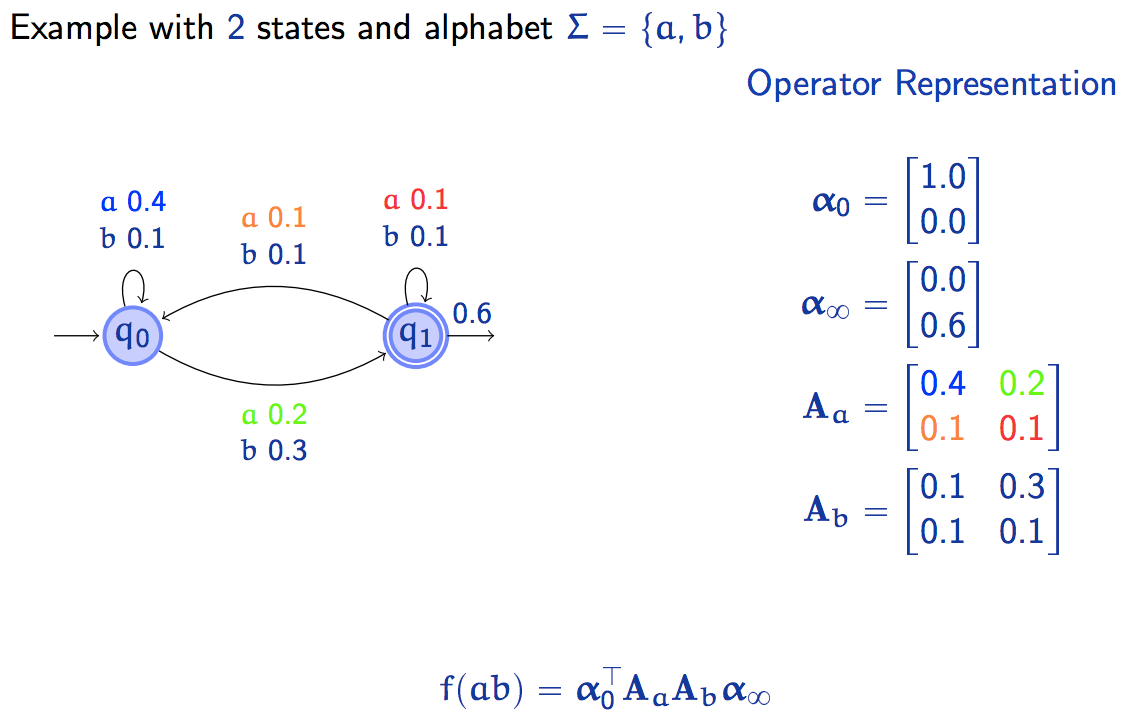
\includegraphics[width=\linewidth]{wfa.png}

$f_{A}(\vek{x}) = f_{A}(x1, ... x_N) = \vek{\alpha_0}^T\vek{A_x}\alpha_{\infty}$

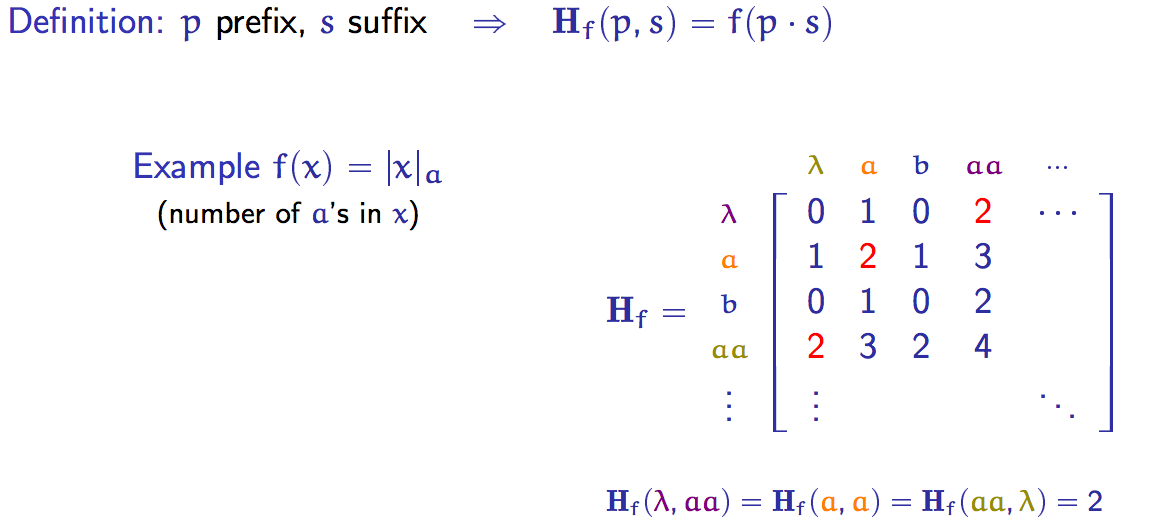
\includegraphics[width=\linewidth]{hankel.png}

If $\text{rank}(H_f) = n$ then there exists WFA $A$ with $n$ states s.t. $f = f_A$.

Estimate hankel matrix from data. Perform SVD of H, solve for parameters with pseudo-inverses. 

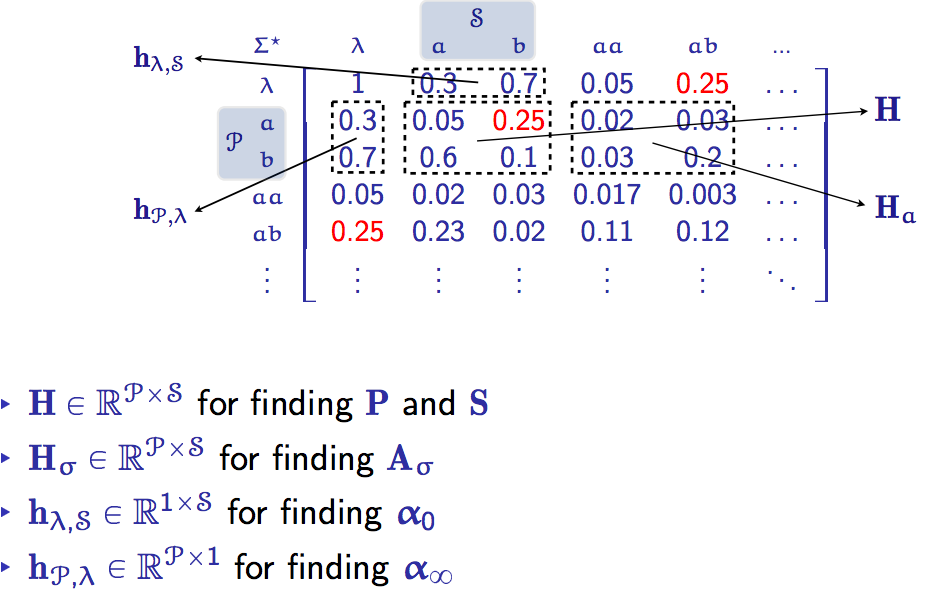
\includegraphics[width=\linewidth]{hankel2.png}

\section{Method of Moments}

Yields consistent estimators (approach true distribution in limit of infinite data) in contrast to EM. Is not subject to local optima. Sample and computational complexity are polynomial.

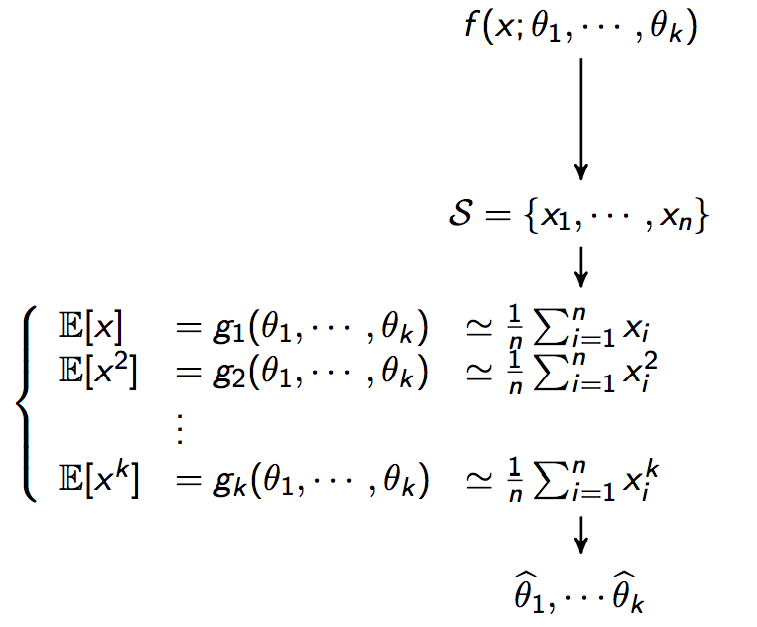
\includegraphics[width=\linewidth]{method_of_moments.png}

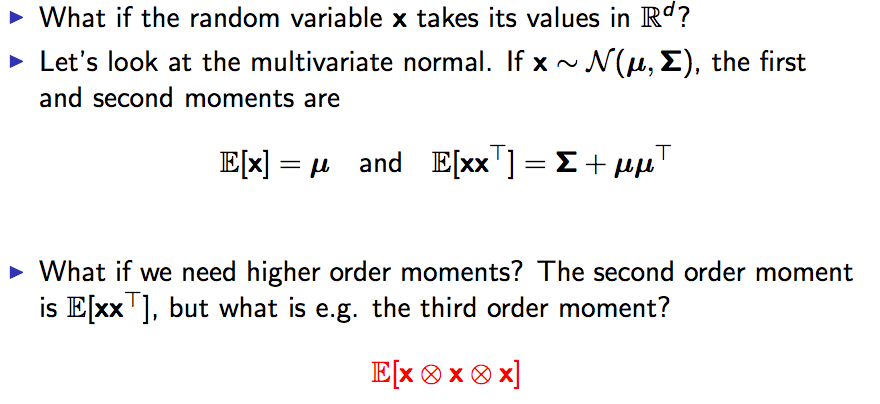
\includegraphics[width=\linewidth]{mom_tensors.png}

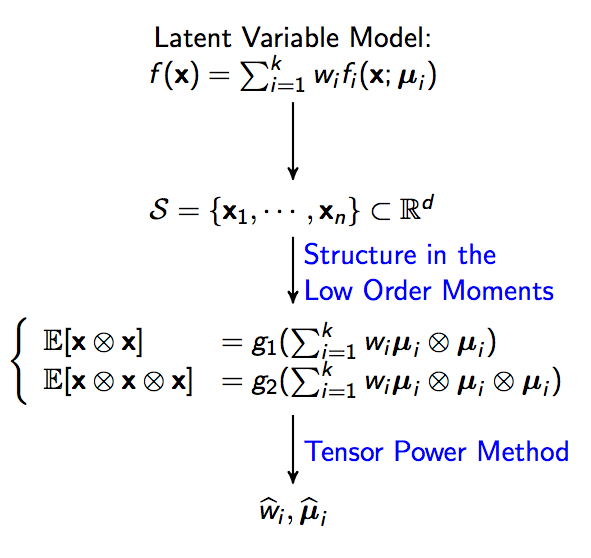
\includegraphics[width=\linewidth]{mom_2.png}

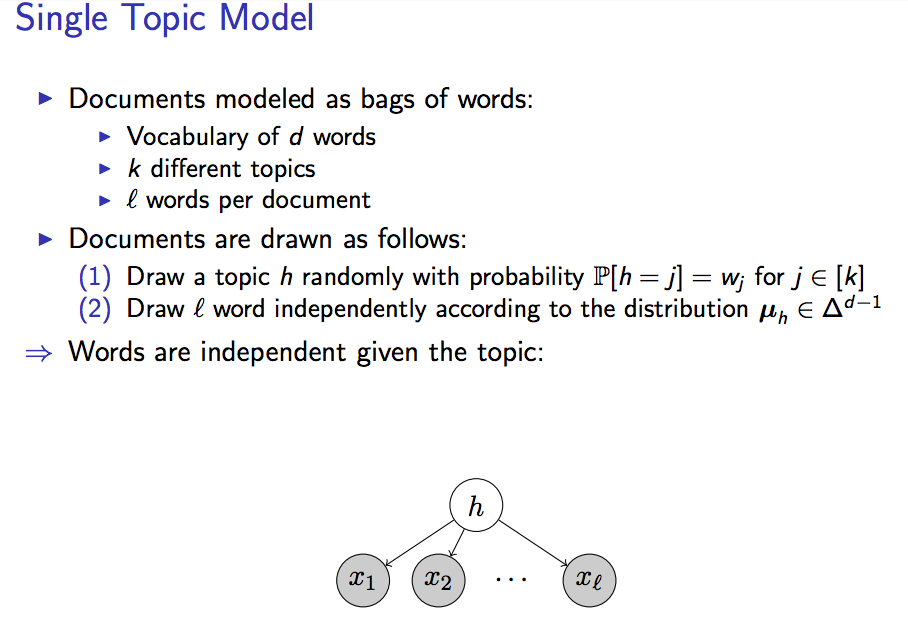
\includegraphics[width=\linewidth]{single_topic.png}

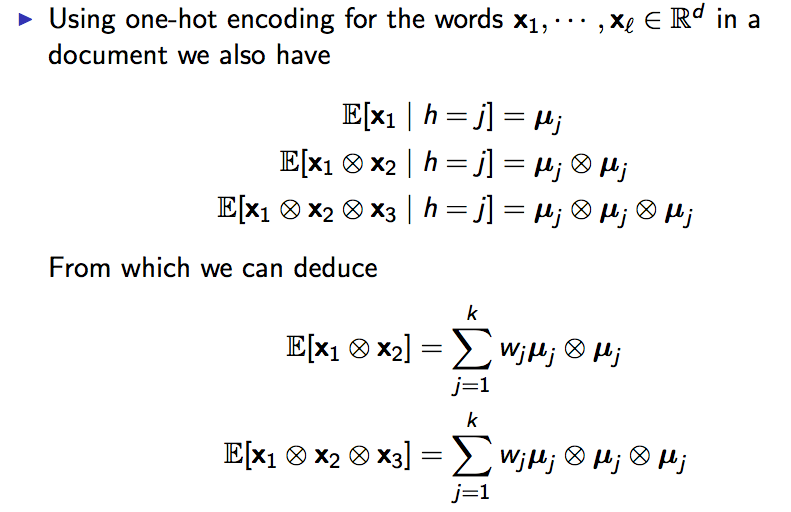
\includegraphics[width=\linewidth]{single_topic_2.png}

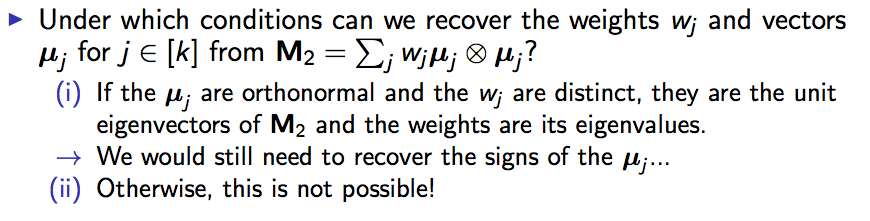
\includegraphics[width=\linewidth]{tensor_decomp.png}

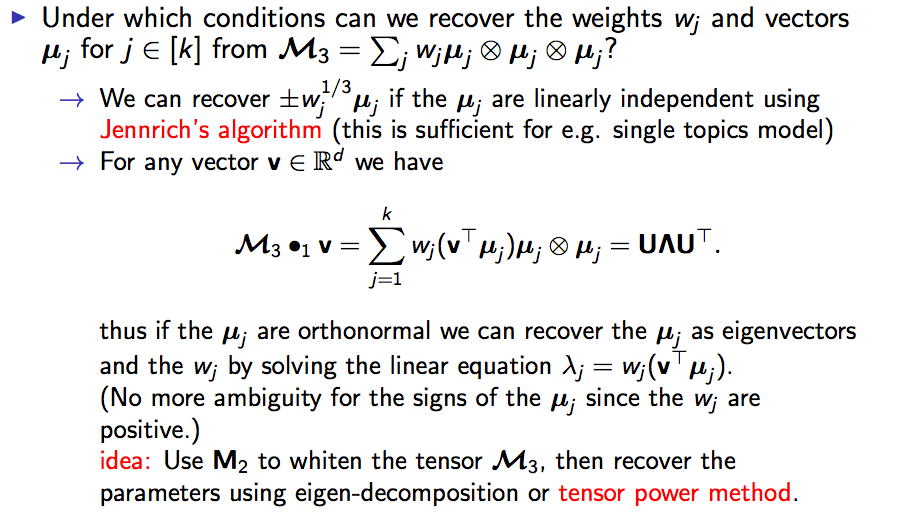
\includegraphics[width=\linewidth]{tensor_decomp_2.png}

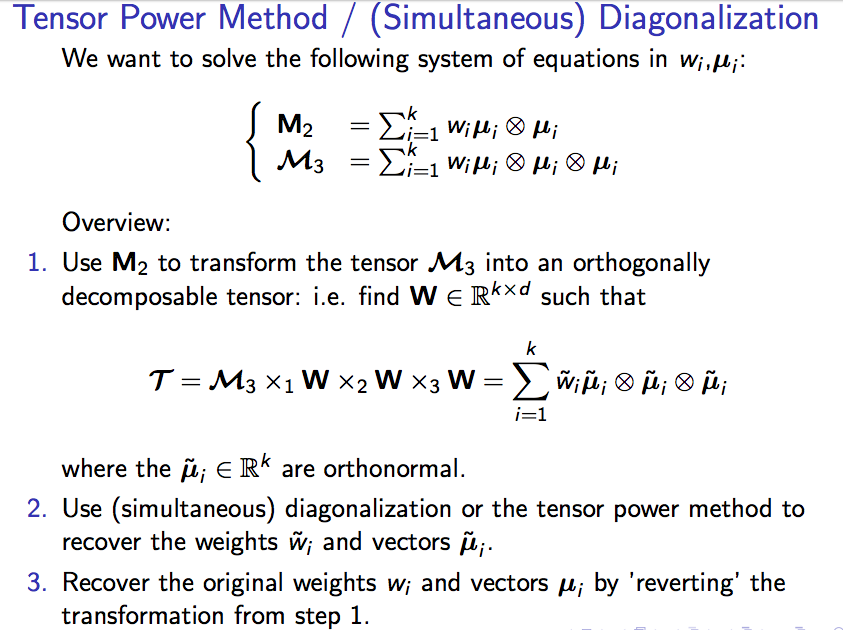
\includegraphics[width=\linewidth]{tensor_decomp_3.png}

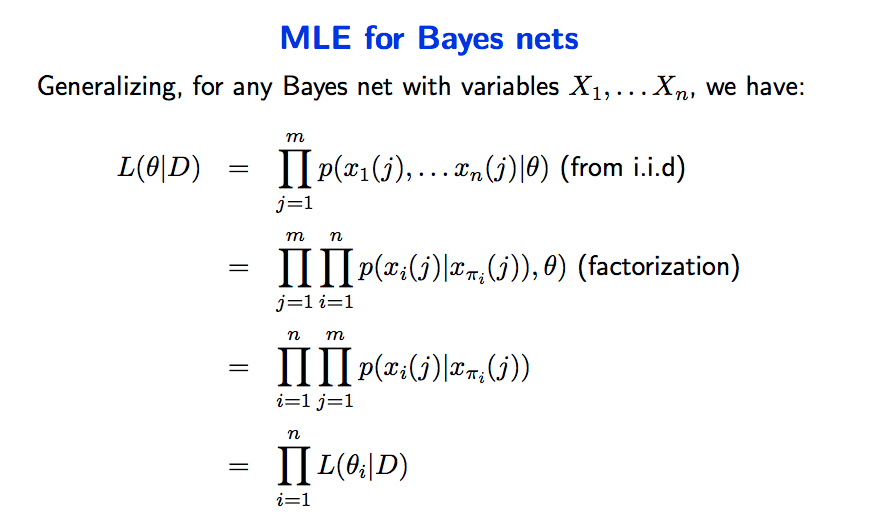
\includegraphics[width=\linewidth]{bayes_mle.png}


\section{HMM notes}
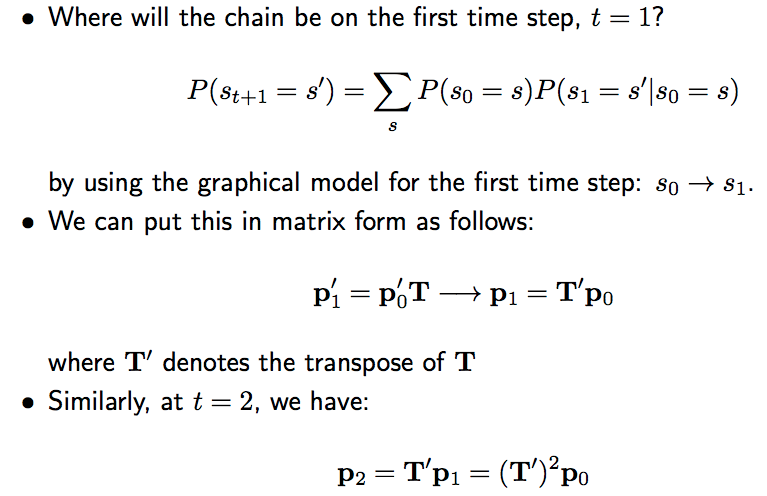
\includegraphics[width=\linewidth]{hmm_2.png}
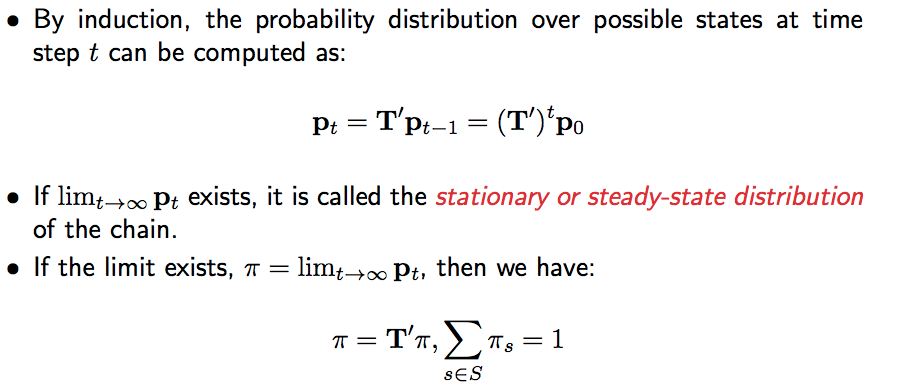
\includegraphics[width=\linewidth]{steady_state.png}

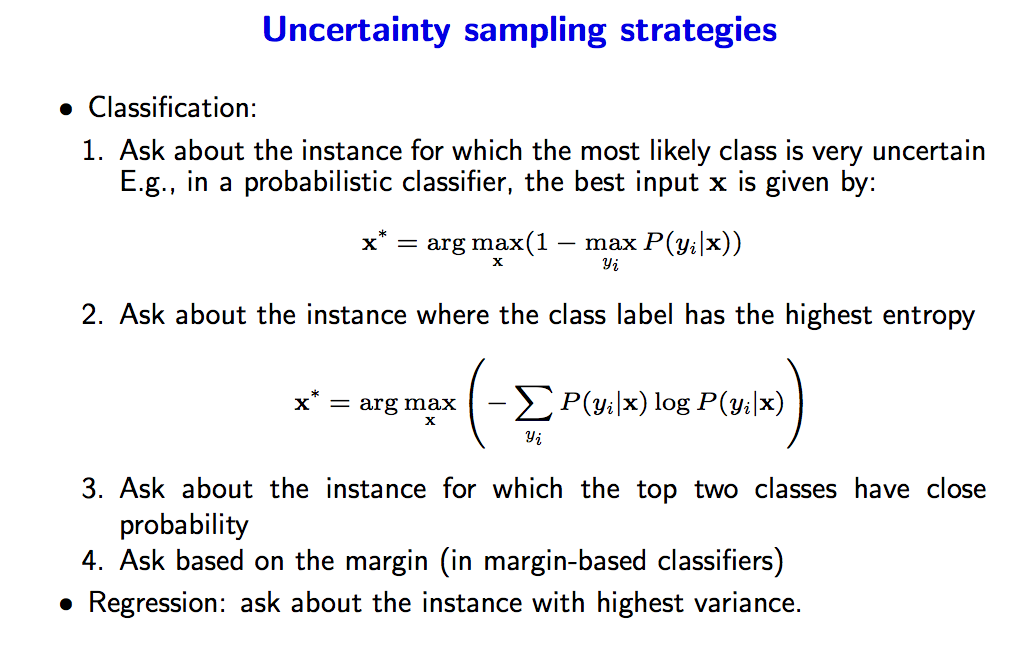
\includegraphics[width=\linewidth]{uncertainty_sampling.png}
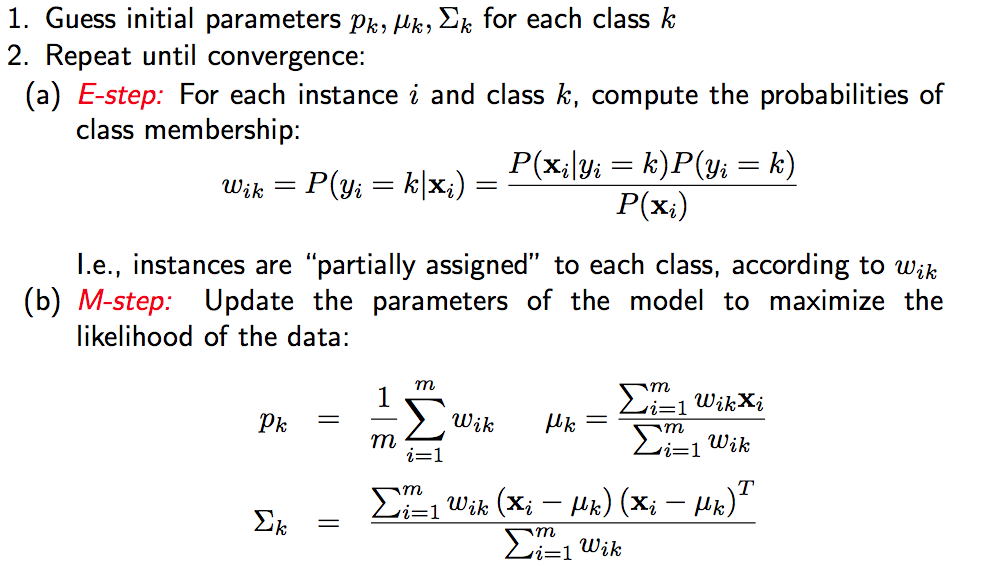
\includegraphics[width=\linewidth]{gauss_soft_em.png}



\section{Miscellaneous}

\begin{itemize}
\item ML overfits as it prefers more parameters. Need regularization.
\item Mean square error is ML estimator of error given gaussian noise assumption.
\item If hypothesis is linear, gradient descent converges to unique global optimum.
\item Gibbs sampling with no evidence: stationary distribution is the joint over all variables.
\item $\frac{P(X = x' \vert y)}{P(X=s \vert y)} = \frac{P(X = x',  y)}{P(X=s, y)} = \frac{\prod_C \psi_C (X = x', y)}{\prod_C \psi_C (X = x, y)}$
\item Bayes net has at most $2^k$ parameters where $k$ is the max number of parents in a node.
\item HMM has unique steady state distribution if it ergodic (all states can be reached from any other state and there are no periodic cycles). Equilibrium reached regardless of initial distribution.
\item Gradient descent not necessarily gives legal parameters.
\end{itemize}




\end{multicols*}
\end{document}